% !TEX root = ../main.tex

\chapter{绪论}

\section{研究背景与意义}

异常检测是金融风控、反欺诈、反洗钱、交易监测与平台治理等场景中的基础能力，其目标是在大量正常样本中识别出少量偏离总体分布的高风险对象。与传统监督学习任务相比，金融异常检测通常面临标签稀缺、异常样本极度不平衡、异常模式持续变化以及业务时效性要求高等现实约束，因此研究重点不仅在于检测模型能否识别出异常，更在于系统能否在真实业务环境中以可接受的吞吐率与时延稳定运行\citep{aggarwal2017outlier,zhao2022tod}。随着金融数据规模从百万级扩展至千万级乃至更高量级，异常检测任务已不再是单纯的模型计算问题，而成为一个包含数据准备、候选检索、异常评分、设备间通信、日志追踪与在线扩展在内的系统工程问题\citep{zhao2022tod,xiao2025flashanns}。

如图~\ref{fig:fin-ad-business-scene} 所示，在金融业务场景中，异常检测通常服务于实时交易风控、支付反欺诈、账户行为审计、洗钱交易排查与交易路径审查等任务。这些场景具有两类显著特征：其一，数据规模大、维度高、更新快，交易行为、账户状态、地理位置、设备指纹、操作轨迹与时间统计特征往往需要共同参与异常判定；其二，系统必须在较短时间内给出可执行的异常评分或告警结果，延迟过高会直接影响业务决策有效性，吞吐不足则会导致高峰期检测链路阻塞\citep{aggarwal2017outlier}。因此，一个面向金融场景的异常检测系统必须同时具备较高计算效率、较低数据路径开销以及良好的工程可扩展性。

传统基于 CPU 的异常检测系统在小规模数据环境下能够完成较为稳定的训练与推理，但当样本规模不断增大时，距离计算、排序、候选组织与统计聚合等操作所带来的时间与空间开销会迅速放大\citep{aggarwal2017outlier,zhao2022tod}，如图~\ref{fig:scale-bottleneck-migration} 所示。近年来研究者开始将 GPU 用于异常检测加速，希望借助并行能力提升距离计算、排序和统计聚合效率。然而，仅对单一算子进行加速并不必然能够构建高性能异常检测系统：随着单算子执行速度提升，系统瓶颈会进一步转移到 CPU$\leftrightarrow$GPU 数据传输、检索与评分阶段间的中间结果组织，以及多 GPU 场景下的任务调度与结果聚合上\citep{faiss_gpu_wiki,rapids_rmm_pinned}。

与此同时，大规模近似最近邻（ANN）检索系统的发展可以成为异常检测系统的新思路。对于金融大规模异常检测任务而言，并不一定需要对全量样本直接执行高代价评分，而可以先借助高吞吐候选召回模块在大规模数据中快速筛出候选集合，再对候选集合执行更精细的异常评分。这种``候选召回---精排评分''的两阶段思路，一方面能够显著降低后续异常评分的计算负担，另一方面也使系统具备更好的吞吐可扩展性\citep{xiao2025flashanns}。然而，在工程实现层面，候选召回与异常评分并不是简单串联即可，还需要解决中间结果表示、跨阶段数据搬运、GPU 内存组织、I/O 与计算重叠以及多 GPU 扩展等一系列问题\citep{xiao2025flashanns,cuvs_multi_gpu_nn}。

基于上述背景，本文选择从系统角度研究金融大规模异常检测问题，聚焦于 PyTOD 与 FlashANNS 的融合实现。PyTOD 通过张量算子抽象支撑异常评分主干，FlashANNS 通过异步 I/O---计算流水线提供高吞吐候选召回能力\citep{zhao2022tod,xiao2025flashanns}。将二者结合，有助于降低全量异常评分的计算负担，并通过统一的数据流、算子流与调度流优化异常检测系统的整体性能。更进一步，在单卡场景中若能构建 GPU 主导端到端执行链路，使查询特征、候选结果与评分中间张量尽量驻留 GPU，则可减少 CPU 与 GPU 间的数据搬运；在多卡场景中若采用数据并行与索引复制，使每张 GPU 独立完成本地闭环，并让 CPU 尽量退出数据平面，仅保留控制面职责，则有望在保持复杂度可控的同时提升整体吞吐\citep{cuvs_multi_gpu_nn,cuvs_dist_mode}。

因此，围绕金融大规模异常检测系统的研究具有明确的理论意义和工程意义：它推动异常检测研究从``单一检测模型优化''向``模型---系统协同优化''发展，并为金融风控场景下构建高吞吐、低时延、可扩展的异常检测系统提供可行路线。


\begin{figure}[htbp]
  \centering
  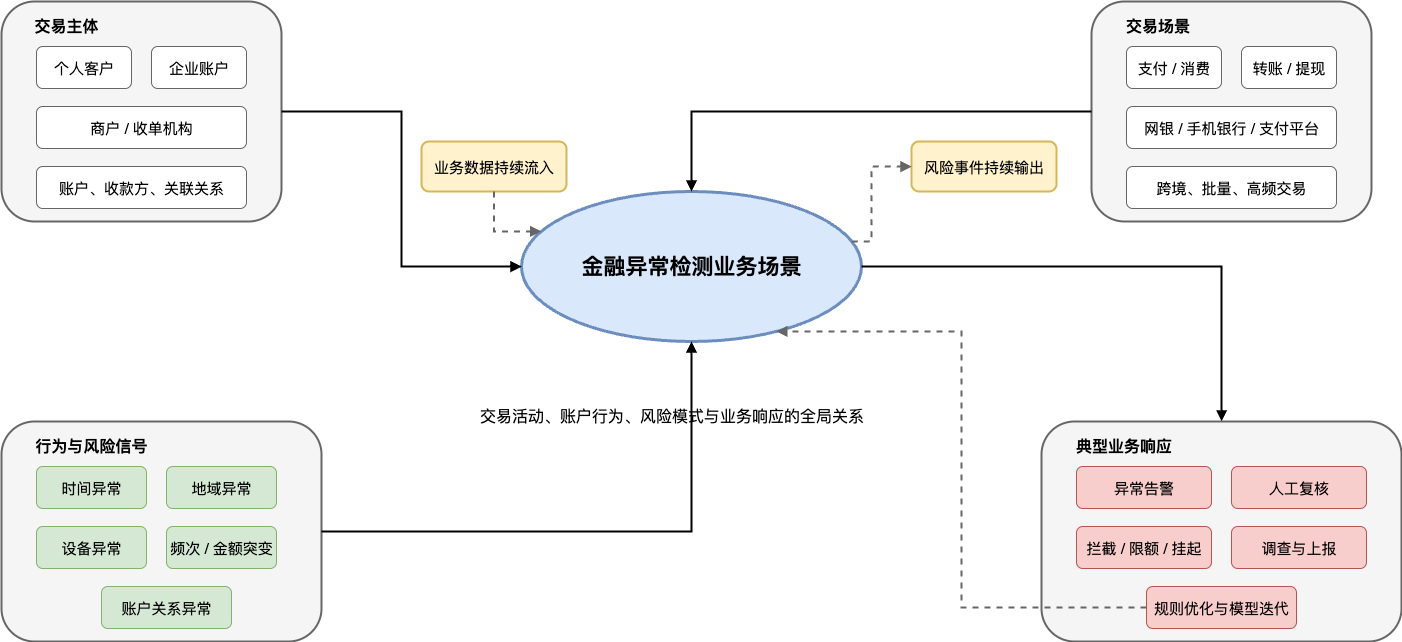
\includegraphics[width=\linewidth]{figures/fig1_1_financial_anomaly_business_scene.png}
  \caption{金融异常检测业务场景总览图}
  \label{fig:fin-ad-business-scene}
\end{figure}

\begin{figure}[htbp]
  \centering
  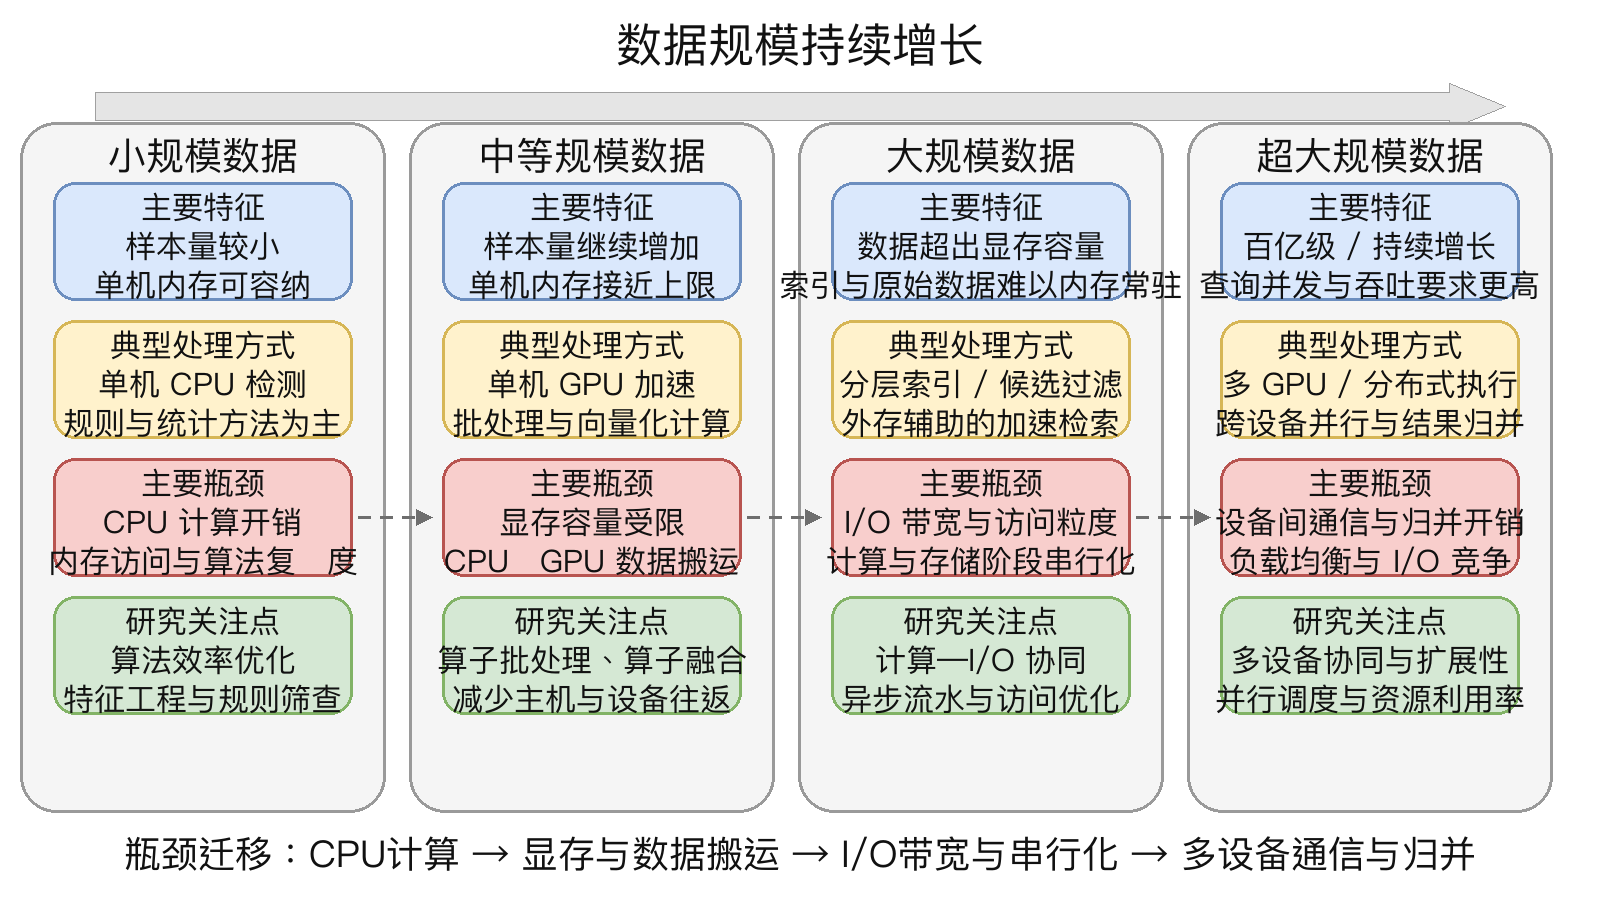
\includegraphics[width=\linewidth]{figures/fig1_2_scale_bottleneck_migration.png}
  \caption{数据规模增长与系统瓶颈迁移示意图}
  \label{fig:scale-bottleneck-migration}
\end{figure}

\section{研究问题与研究对象}

金融大规模异常检测任务的核心，在于对大量交易、账户与行为记录进行快速筛查，并在保证检测效果的前提下及时输出异常分数或告警结果，如图~\ref{fig:fin-ad-standard-flow} 所示。与传统离线分析任务不同，金融场景中的异常检测往往具有连续到达、时延敏感和峰值流量显著等特点，这使得系统必须在有限时间内完成特征构造、候选检索、异常评分与结果输出等多个阶段\citep{aggarwal2017outlier}。由于不同阶段的计算模式、数据访问模式和资源需求各不相同，因此本文将研究对象定义为一个完整的异常检测系统，而非某一个独立的异常检测算法。

从任务流程上看，本文关注的系统可抽象为如下处理链路：对输入的金融交易记录、账户行为统计和上下文特征进行规范化与向量化表示；基于向量化表示执行高吞吐候选召回，以缩小后续异常评分所需处理的样本范围；在候选集合上执行张量化异常评分，输出异常分数或排序结果；结合日志、统计指标与告警规则完成结果输出与追踪\citep{zhao2022tod,xiao2025flashanns}。

围绕这一系统处理流程，本文选择 \textbf{PyTOD--FlashANNS 融合异常检测系统} 作为研究对象。PyTOD 的优势在于将异常检测过程抽象为一组可复用的张量算子，使距离计算、排序、聚合与统计过程能够在 GPU 上以统一语义执行；FlashANNS 的优势则在于为大规模候选召回提供异步 I/O---计算流水线和高吞吐检索能力，如图~\ref{fig:pytod-flashanns-concept} 所示\citep{zhao2022tod,xiao2025flashanns}。

然而，PyTOD 与 FlashANNS 的简单串联并不能自动得到高性能系统。若查询特征在 CPU 上构造，再传输至 GPU 进行候选检索，而候选结果又返回 CPU 重新组织后再送回 GPU 评分，则系统瓶颈将从算子执行转移到 CPU$\leftrightarrow$GPU 数据搬运与阶段同步上\citep{faiss_gpu_wiki,rapids_rmm_pinned}。进一步地，在多 GPU 场景中，若采用索引分片并将多个 GPU 上的局部结果集中到 CPU 归并，则 CPU 可能重新成为系统瓶颈\citep{cuvs_multi_gpu_ivf_host}。

基于此，本文的研究问题可归纳为以下四点：
\begin{enumerate}
  \item 如何将 PyTOD 的张量化异常评分能力与 FlashANNS 的高吞吐候选召回能力有机结合，构建统一的金融异常检测执行链路；
  \item 如何在单卡场景中构建 GPU 主导的端到端执行链路，使查询特征、候选结果与评分中间张量尽量保持在 GPU 侧，从而减少 CPU 与 GPU 之间的非必要往返与 I/O 串行等待；
  \item 如何在多 GPU 场景下优先采用数据并行与索引复制策略，使每张 GPU 独立完成候选召回与异常评分，降低 CPU 聚合和跨卡通信对系统吞吐的影响；
  \item 当索引容量或业务约束导致必须跨卡归并时，如何将归并逻辑尽量下沉至 GPU 并通过 NCCL 等设备间通信机制完成结果合并，同时结合拓扑感知的 I/O lane 绑定与准入控制避免共享存储路径成为新瓶颈\citep{nccl_stream_semantics,gds_overview}。
\end{enumerate}

因此，本文的研究对象不是单一``异常检测模型''，也不是单一``向量检索组件''，而是一个面向金融大规模异常检测任务的融合系统。本文重点回答的问题是：\textbf{如何在保证检测效果可接受的前提下，将候选召回、异常评分、数据路径优化和多 GPU 扩展统一到一个可部署、可扩展、可验证的系统框架中。}


\begin{figure}[htbp]
  \centering
  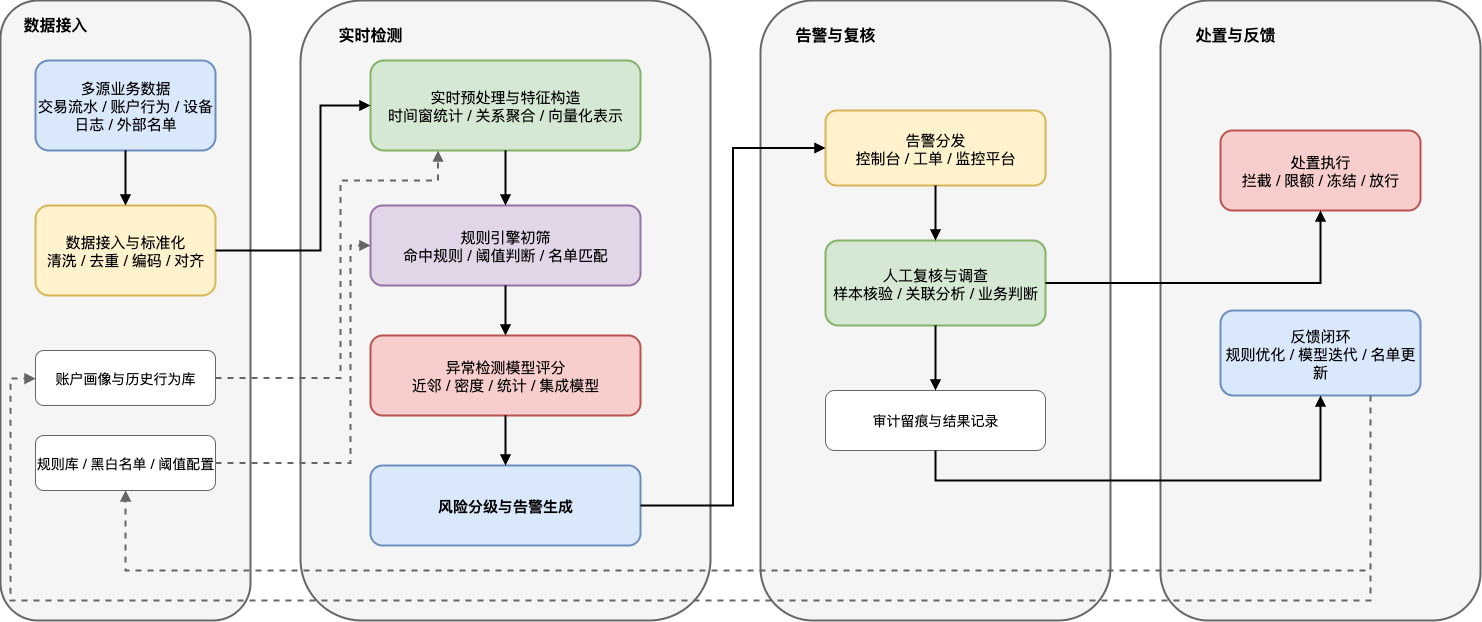
\includegraphics[width=\linewidth]{figures/fig1_3_financial_anomaly_standard_flow.png}
  \caption{金融大规模异常检测系统标准处理流程图}
  \label{fig:fin-ad-standard-flow}
\end{figure}

\begin{figure}[htbp]
  \centering
  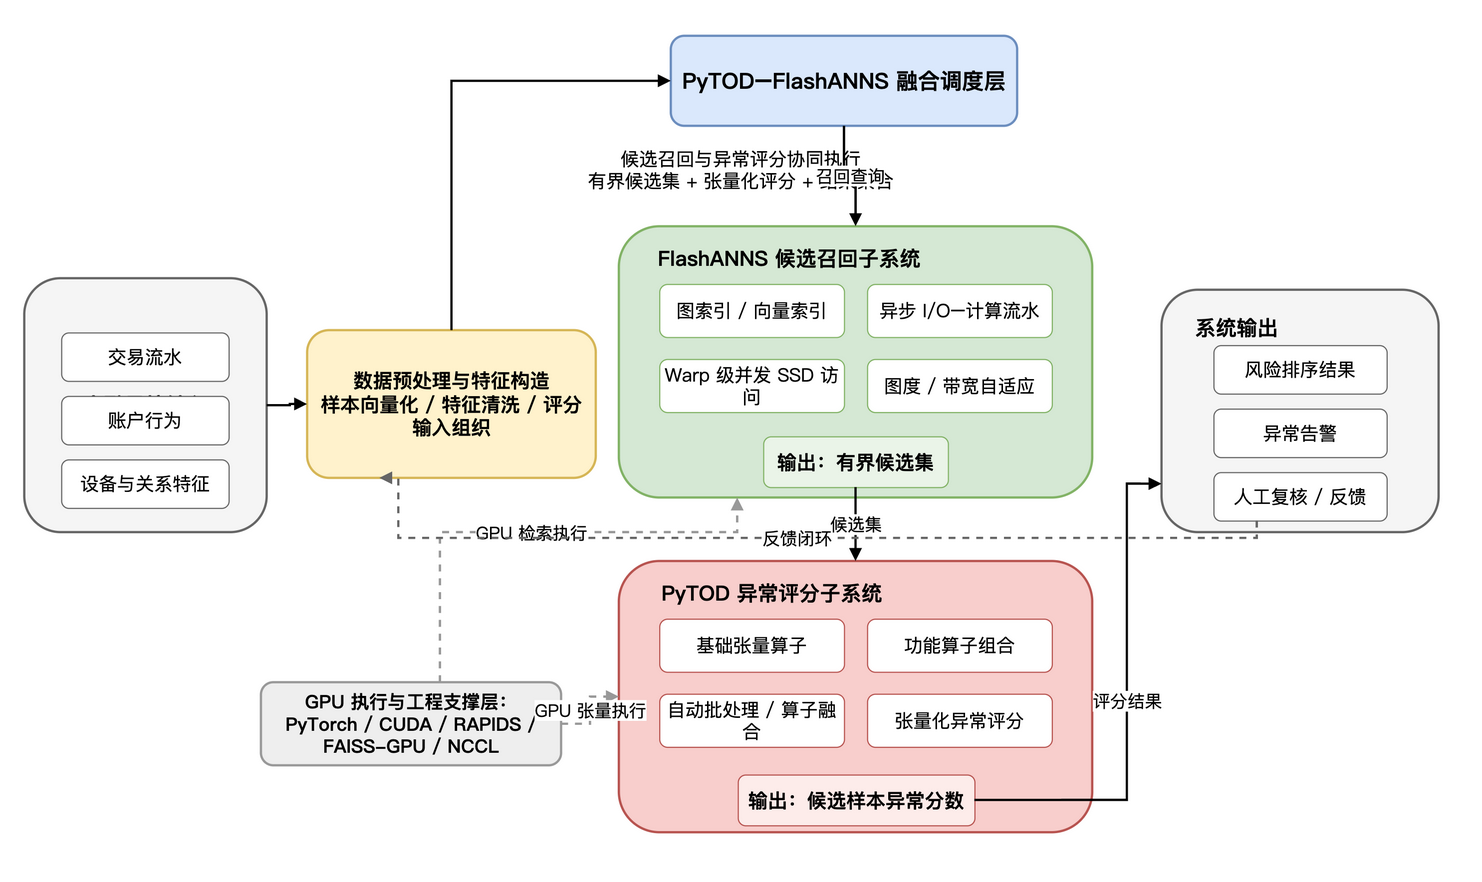
\includegraphics[width=0.95\linewidth]{figures/fig1_4_pytod_flashanns_concept.png}
  \caption{PyTOD--FlashANNS 融合系统概念图}
  \label{fig:pytod-flashanns-concept}
\end{figure}

\section{核心问题分析}

对于面向金融场景的大规模异常检测系统，性能瓶颈并不来自单一环节，而是由异常评分复杂度、候选召回开销、数据路径组织成本以及多 GPU 扩展代价共同决定。为明确本文研究重点，本节对核心问题进行分析。

\subsection{异常评分阶段的高复杂度计算问题}

许多异常检测方法依赖样本之间的距离、近邻关系或统计偏离程度进行评分，尤其是基于近邻、密度或局部异常因子的检测方法，需要大量距离计算、排序与聚合操作\citep{aggarwal2017outlier,breunig2000lof}。当数据规模上升到百万级以上时，全量距离矩阵的显式构造会带来极高计算开销与内存压力。PyTOD 通过张量算子抽象提升异常评分计算效率\citep{zhao2022tod}，但其优势主要体现在``如何高效计算评分''，而非``如何缩小评分对象范围''，因此评分复杂度必须与候选召回联合考虑。

\subsection{候选召回阶段的存储访问与吞吐瓶颈问题}

候选召回为后续评分提供规模可控且质量可接受的候选集合\citep{xiao2025flashanns}。在大规模数据环境中，当索引规模超过显存容量并进入 out-of-core 路径时，I/O 与计算协同效率成为吞吐上限的关键因素。FlashANNS 的异步 I/O---计算流水线证明，通过重叠 SSD 访问与 GPU 计算可显著提升持续吞吐\citep{xiao2025flashanns}。

\subsection{CPU--GPU 数据传输与阶段同步问题}

在工程系统中，瓶颈往往来自阶段边界的数据组织、格式转换与同步等待。若查询特征与候选结果频繁在 CPU 与 GPU 之间往返，即便候选召回和异常评分算子已被加速，端到端吞吐仍会被 H2D/D2H 与阶段同步拖慢\citep{faiss_gpu_wiki,rapids_rmm_pinned}。

\subsection{多 GPU 扩展中的结果聚合与共享 I/O 瓶颈问题}

多 GPU 扩展并不必然线性：一方面存在索引复制、查询分发、设备间通信与归并开销；另一方面多卡并发访问共享 PCIe/NUMA/SSD 可能放大 I/O 竞争\citep{cuvs_multi_gpu_nn,gds_overview}。因此，多 GPU 扩展的核心问题是如何在保持复杂度可控前提下提升吞吐，并避免 CPU 聚合与共享 I/O 再次成为瓶颈。


\section{研究目标与技术路线}

本文的研究目标是在保证异常检测效果可接受的前提下，构建一套面向大规模金融数据运行、具备较高吞吐率、较低时延并支持多 GPU 扩展的融合异常检测系统。围绕该目标，本文从系统架构、单卡数据路径优化和多卡扩展机制三个层面展开研究。系统的整体技术路线图如图~\ref{fig:technical-route} 所示。

系统功能层面，以 PyTOD 为异常评分主干、以 FlashANNS 为候选召回模块，建立二阶段执行结构：通过候选召回缩小评分范围，再在候选集合上执行张量化异常评分\citep{zhao2022tod,xiao2025flashanns}。

单卡性能优化层面，提出 GPU 主导端到端执行链路：在 FlashANNS 异步 I/O---计算流水线基础上，使查询特征、候选结果与评分中间张量尽量保持在 GPU 侧，仅在必要边界通过 pinned memory 与主机交互；并引入 RAPIDS 与 FAISS-GPU 进行后端增强\citep{rapids_cudf_pandas,faiss_gpu_wiki,rapids_rmm_pinned}。

多 GPU 扩展层面，优先采用数据并行与索引复制策略，使每张 GPU 独立完成本地闭环，CPU 仅保留控制面职责；当索引无法复制时，采用 GPU 侧归并与 NCCL 通信作为兜底，并结合拓扑感知 I/O lane 控制降低共享路径冲突\citep{cuvs_multi_gpu_nn,nccl_stream_semantics,gds_design_guide}。

\begin{figure}[htbp]
  \centering
  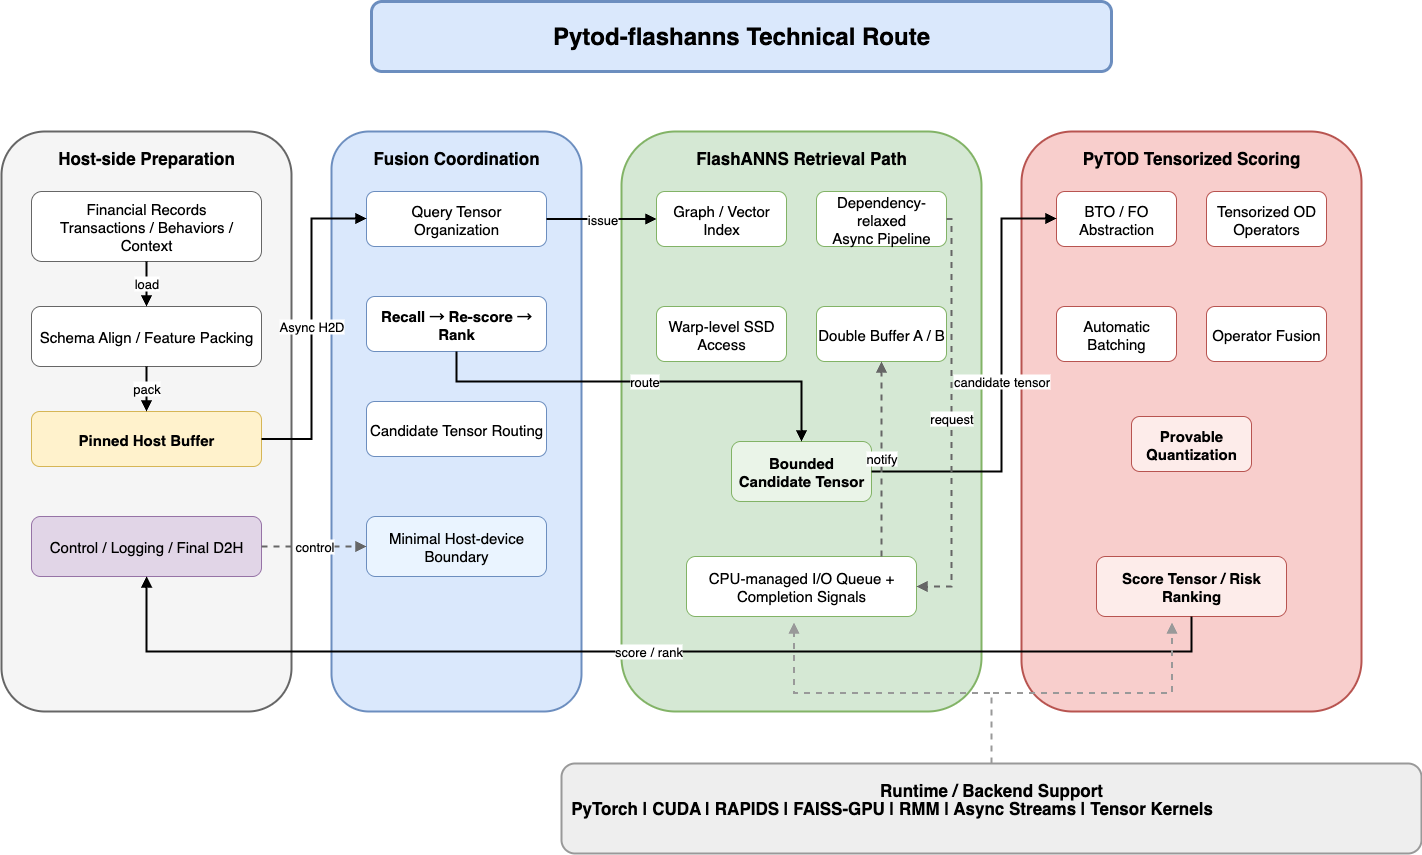
\includegraphics[width=\linewidth]{figures/fig1_7_pytod_flashanns_technical_route.png}
  \caption{全文技术路线图}
  \label{fig:technical-route}
\end{figure}

\section{本文主要工作与创新点}

本文主要工作包括：构建 PyTOD--FlashANNS 融合框架；提出单卡 GPU 主导端到端执行链路并进行数据路径压缩；引入 RAPIDS 与 FAISS-GPU 重组数据处理与检索后端；提出多 GPU 数据并行与索引复制主方案，并给出 GPU 侧归并与拓扑感知 I/O 控制兜底机制\citep{zhao2022tod,xiao2025flashanns,cuvs_multi_gpu_nn}。

本文创新点概括为三方面：
\begin{enumerate}
  \item \textbf{系统融合创新：}提出面向金融异常检测任务的 PyTOD--FlashANNS 融合架构，构建候选召回---异常评分协同执行链路；
  \item \textbf{单卡数据路径优化创新：}提出 GPU 主导端到端执行链路，在异步 I/O---计算流水线基础上压缩 CPU$\leftrightarrow$GPU 数据路径，并结合 RAPIDS/FAISS-GPU/pinned memory/异步流降低整体开销；
  \item \textbf{多 GPU 扩展创新：}提出数据并行与索引复制的多 GPU 扩展策略，使 CPU 退出数据平面；在必要时引入 GPU 侧跨卡归并、NCCL 通信与拓扑感知 I/O 优化支撑更复杂场景。
\end{enumerate}


\section{论文组织结构}

全文围绕``问题提出---相关研究---融合模型构建---单卡系统优化---多 GPU 扩展---综合实验验证---总结展望''的逻辑展开，各章内容如下：第一章为绪论；第二章为相关研究工作与关键技术基础；第三章为融合检测模型与数据准备；第四章为单卡系统设计与数据路径优化；第五章为多 GPU 扩展与聚合优化；第六章为综合实验与讨论；第七章为全文总结与展望。
